\definecolor{singleShotColor}{RGB}{196,106,28}
\definecolor{pipelineColor}{RGB}{44,138,100}
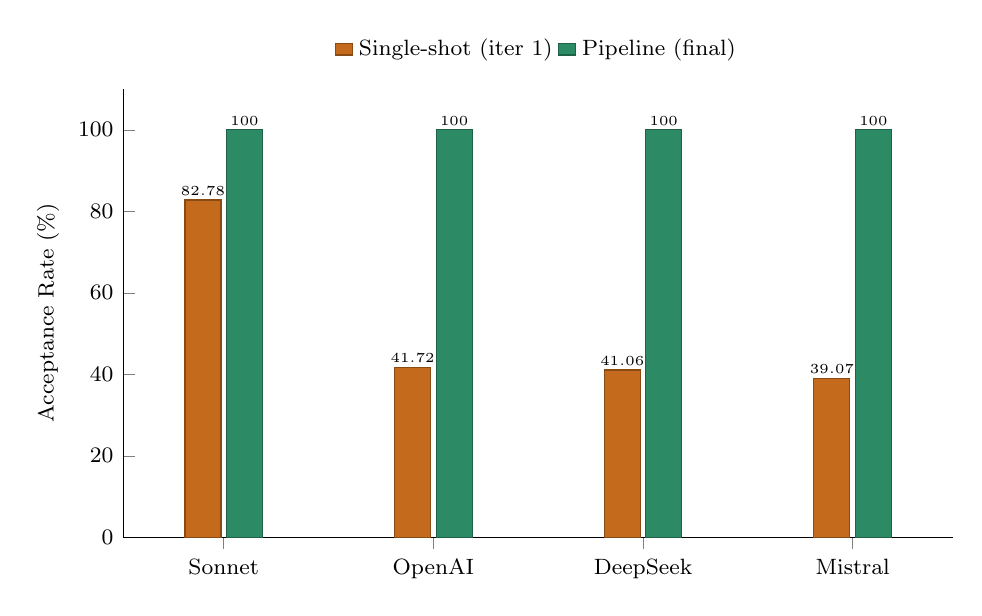
\begin{tikzpicture}
\begin{axis}[
    ybar,
    bar width=13pt,
    width=\columnwidth,
    height=0.60\columnwidth,
    ymin=0,
    ymax=110,
    ylabel={Acceptance Rate (\%)},
    symbolic x coords={Sonnet,OpenAI,DeepSeek,Mistral},
    xtick=data,
    xticklabel style={font=\footnotesize, rotate=0, anchor=north},
    nodes near coords,
    nodes near coords={\pgfmathprintnumber[fixed,precision=2]{\pgfplotspointmeta}},
    nodes near coords align={center},
    nodes near coords style={
        font=\tiny,
        text=black,
    },
    every node near coord/.append style={anchor=south, yshift=-1.8pt},
    ymajorgrids=false,
    enlarge x limits=0.16,
    axis lines*=left,
    tick label style={font=\footnotesize},
    label style={font=\footnotesize},
    legend style={
        draw=none,
        font=\footnotesize,
        at={(0.5,1.04)},
        anchor=south,
        legend columns=2
    },
    legend cell align={left},
    legend image code/.code={
        \draw[#1] (0cm,-0.075cm) rectangle (0.22cm,0.075cm);
    },
]
\addplot+[fill=singleShotColor, draw=singleShotColor!70!black] coordinates {
    (Sonnet,82.78)
    (OpenAI,41.72)
    (DeepSeek,41.06)
    (Mistral,39.07)
};
\addplot+[fill=pipelineColor, draw=pipelineColor!70!black] coordinates {
    (Sonnet,100.00)
    (OpenAI,100.00)
    (DeepSeek,100.00)
    (Mistral,100.00)
};
\legend{Single-shot (iter 1),Pipeline (final)}
\end{axis}
\end{tikzpicture}
